\section{Constraints from Non-collider Searches}

Beyond the collider experiments, low-energy experiments and astrophysical observation also help to constrain the parameter space of LLPs. A variety of observations and experiments have been made or proposed, and only some indirect observations for milli-Charged Particle (mCP) are discussed in this section as demonstrations. A new fermion mCP is introduced along with an additional $U(1)$ gauge symmetry, which couples to normal photon via a fractional coupling $\epsilon e$. Further details about mCP can be found in following section. A summary of cosmological and astrophysical constraints for mCP is shown in Fig.\ref{fig:mCPnoncollider}:
\begin{figure}[!h]
    \centering
    \caption{Summary of cosmological and astrophysical constraints for mCP spanned by fractional charge $\epsilon = Q/e$ and mass of mCP $m_\epsilon$. From Ref.\cite{mCPnoncollider}}
    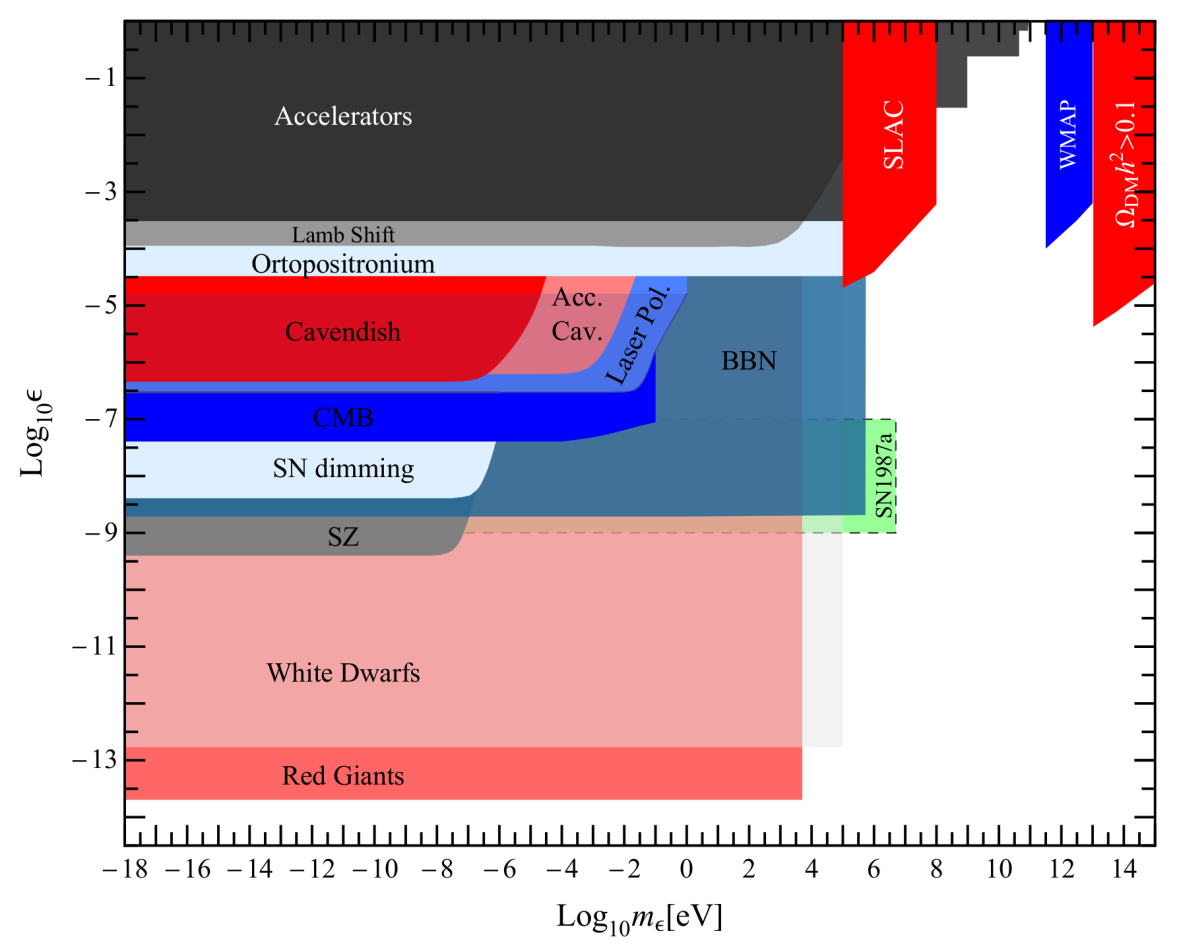
\includegraphics[width=0.5\textwidth]{fig/noncolliderMCP.png}
    \label{fig:mCPnoncollider}
\end{figure}
Lamb shift of hydrogen atom are investigated with effect of milli-charged particle \cite{mCPlambshift}. The existence of mCP will contribute to lamb shift via vacuum polarization (VP) term
\begin{equation}
    \delta E_{VP} = -\frac{4\alpha^3 m_e}{3\pi}\epsilon^2 \alpha^{\ast 2}I(\alpha^{\ast})
\end{equation}
where $I(\alpha^{\ast})$ defined as:
\begin{equation}
    I(\alpha^{\ast}) = \int^{\infty}_{0}du(1+\frac{1}{2u^2})\frac{\sqrt{u^2-1}}{(\alpha^{\ast}+2u)^4}
\end{equation}
with the effective coupling $\alpha^{\ast} = \alpha m_e/M_{mCP}$. Corresponding to the a $1\sigma$ discrepancy between the measured and calculated shifts, leading order polarization contribution $|\delta E_{VP}|/2\pi\hbar$ from mCP to the Lamb shift should be less than 0.01 MHz. The upper bound on mCP are then $\epsilon \leq 1.085\times10^{-4}$ for $M_{mCP} \lesssim 1 keV$.


One of the major observations is Big-Bang Nucleosynthesis (BBN), charged particle will interact with the plasma in the early universe and get thermally excited. Hence the existence of additional light charged particle will affect the effective number of (nearly) massless neutrino flavor $N_{eff}$, which reported by $Planck$ 2015 result to be $N_{eff}^{CMB} = 3.13 \pm 0.31$ thus tightly constraining non-standard nucleosynthesis scenario. The effect of the milli-charged particles are calculated numerically in \cite{mCPwithBBN} as:
\begin{equation}
    \Delta N_{eff} = 0.69 \times 10^{17} \epsilon^2 \times \begin{cases}
               1 &\text{no elastic scattering,}\\
               1.39 &\text{full equilibrium,}\\
            \end{cases}
\end{equation}
Then BBN implies a limit
\begin{equation}
    \epsilon < 2.5 \times10 ^{-9}
\end{equation}
This bound applies to masses in the regime $m_{mCP} \lesssim m_e$.
Constraints from the cosmic microwave background (CMB), accurate measurements in low-energy experiments and many other astrophysical systems are described in \cite{mCPCMB,mCPCMB2,mCPnoncollider,mCPlambshift,mCPcosmology,mCPastro,mCPaccecavity,mCPPositronium,mCPLaser,mCPHubble,mCPCoulomb}.